\documentclass[3p,twocolumn,10pt]{elsarticle}
\setlength{\footskip}{30pt}

%% Use the option review to obtain double line spacing
%% \documentclass[authoryear,preprint,review,12pt]{elsarticle}

%% Use the options 1p,twocolumn; 3p; 3p,twocolumn; 5p; or 5p,twocolumn
%% for a journal layout:
%% \documentclass[final,1p,times]{elsarticle}
%% \documentclass[final,1p,times,twocolumn]{elsarticle}
%% \documentclass[final,3p,times]{elsarticle}
%% \documentclass[final,3p,times,twocolumn]{elsarticle}
%% \documentclass[final,5p,times]{elsarticle}
%% \documentclass[final,5p,times,twocolumn]{elsarticle}

%% For including figures, graphicx.sty has been loaded in
%% elsarticle.cls. If you prefer to use the old commands
%% please give \usepackage{epsfig}

\usepackage[utf8]{inputenc}
\usepackage[T1]{fontenc}
\usepackage{lmodern}
\usepackage{tgpagella}

% Extensive support for hypertext.
\usepackage[hidelinks,colorlinks=true]{hyperref}

% Easy access to the Lorem Ipsum dummy text.
\usepackage{lipsum}

% Pro­vides both fore­ground (text, rules, etc.) and back­ground colour man­age­ment.
\usepackage{color}

% Driver-independent color extensions.
\usepackage[x11names]{xcolor}

% Enhanced support for graphics.
\usepackage{graphicx}

% Produces figures which text can flow around.
\usepackage{wrapfig}

% Customising captions in floating environments.
\usepackage{caption}

% Publication quality tables.
\usepackage{booktabs}

% Long tables.
\usepackage{longtable}

%% The amssymb package provides various useful mathematical symbols.
%\usepackage{amssymb}

%% The amsthm package provides extended theorem environments.
%\usepackage{amsthm}

%% The lineno packages adds line numbers. Start line numbering with
%% \begin{linenumbers}, end it with \end{linenumbers}. Or switch it on
%% for the whole article with \linenumbers.
%% \usepackage{lineno}

\journal{Journal Name}

% Configure caption display.
\captionsetup{margin=10pt,font=small,labelfont=bf,labelsep=period}

% Define where the images can be found.
\DeclareGraphicsExtensions{.pdf,.png,.jpg}
\graphicspath{{./images/}}

% Define some commands.
\input{db-stats.inc}

\begin{document}

% Configure hyperlink colors after document start to override possible
% documentclass defaults.
\hypersetup{
    citecolor=DodgerBlue4,
    filecolor=DodgerBlue4,
    linkcolor=DodgerBlue4,
    urlcolor=DodgerBlue4
}

\begin{frontmatter}

%% Title, authors and addresses

%% use the tnoteref command within \title for footnotes;
%% use the tnotetext command for the associated footnote;
%% use the fnref command within \author or \address for footnotes;
%% use the fntext command for the associated footnote;
%% use the corref command within \author for corresponding author footnotes;
%% use the cortext command for the associated footnote;
%% use the ead command for the email address,
%% and the form \ead[url] for the home page:
%% \title{Title\tnoteref{label1}}
%% \tnotetext[label1]{}
%% \author{Name\corref{cor1}\fnref{label2}}
%% \ead{email address}
%% \ead[url]{home page}
%% \fntext[label2]{}
%% \cortext[cor1]{}
%% \address{Address\fnref{label3}}
%% \fntext[label3]{}

\title{Automated identification of slipper orchids using image analysis and artificial neural networks}

%% use optional labels to link authors explicitly to addresses:
%% \author[label1,label2]{}
%% \address[label1]{}
%% \address[label2]{}


\author[nbc]{Serrano Pereira}
\author[nbc,hsl,lu]{Barbara Gravendeel}
\author[hsl]{Patrick Wijntjes}
\author[nbc]{Rutger Vos}
\address[nbc]{Naturalis Biodiversity Center, P.O. Box 9517, Leiden, The Netherlands}
\address[hsl]{University of Applied Sciences Leiden, P.O. Box 382, Leiden, The Netherlands}
\address[lu]{Institute Biology Leiden, Leiden University, P.O. Box 546, Leiden, The Netherlands}

% Dave Roberts co-author?

\begin{abstract}
A generic hierarchical identification system was developed for the automated identification of species by image recognition. The effectiveness of this system was assessed using photographs of orchids of the subfamily Cypripedioideae. Colour and shape features were extracted from single flower photos of {\SpeciesCount} orchid species. Generic image preprocessing, segmentation, and feature extraction algorithms were implemented to obtain morphometric data for the different orchid species. The identification system uses a hierarchy of artificial neural networks for pattern recognition and automated classification. The neural network hierarchy mirrors the taxonomic hierarchy of the Cypripedioideae, such that user-submitted photos could be assigned a genus, section, and species classification. The ability of the identification system to correctly identify user-submitted photos varied depending on the photo quality, the number of species included for training, and the desired taxonomic level for identification. High quality photos were scarce for some taxa and were under-represented in the training set, resulting in imbalanced network training. The simple colour features used for training were not sufficient to reliably identify photos to the correct section and species, and more specialised feature extraction algorithms need to be developed to improve accuracy.
\end{abstract}

\begin{keyword}
%% keywords here, in the form: keyword \sep keyword

Cypripedioideae \sep feature extraction \sep identification \sep image analysis
\sep neural networks \sep orchids \sep pattern recognition \sep taxonomy

%% PACS codes here, in the form: \PACS code \sep code

%% MSC codes here, in the form: \MSC code \sep code
%% or \MSC[2008] code \sep code (2000 is the default)
\end{keyword}

\end{frontmatter}

%% \linenumbers

%% main text
\section{Introduction}
\label{sect:introduction}

Ongoing advances in computer vision and machine learning has lead to the development of numerous semi- or fully automated species identification systems. Such systems have been successful in the identification of plant species \citep{Arinkin2014, Nilsback2008, Sanz2013}, phytoplankton \citep{Boddy1994}, diatom frustules \citep{Kloster2014}, and insects \citep{Weeks1999,Kang2012}, amongst others. Artificial Neural Networks (ANNs) in particular have become an increasingly popular choice in automated image classification systems \citep{Weeks1997}.

\lipsum[1]

\section{Materials and methods}
\label{sect:methods}

\subsection{Reference photo collection}

A collection of reference photos was compiled by searching the internet for images, mostly through Google Image searches. The correct genus, section, and species for each image was verified by specialists and referenced to the literature \citet{Cribb1998, Pridgeon1999, Frosch2012} and phylogenetic reconstructions based on molecular analyses \citep{Li2011, Chochai2012}. Every photo was subsequently uploaded to an account on the online image hosting service Flickr (\url{https://www.flickr.com}). On Flickr, each image was annotated with standardized tags in the formats \texttt{genus:name}, \texttt{section:name}, and \texttt{species:name}. A custom Python script utilizing the Flickr API was used to download the entire image collection with metadata from the Flickr account to a local computer, where images are stored in a directory hierarchy and image annotations are stored in a database (\ref{sect:meta-database}).

\subsection{Image feature extraction}

Several feature extraction and neural network training routines were implemented and released as a set of Python scripts (\url{https://github.com/naturalis/nbclassify}). The scripts implement a separate Python package called ImgPheno (\url{https://github.com/naturalis/imgpheno}), which is a collection of several image feature extraction methods. They make use of OpenCV \citep{Pulli2012} for computer vision functionality and NumPy \citep{VanderWalt2011} for array and matrix manipulation functionalities. Feature extraction was automated with a Python script that is executed from the command-line. Configurations are kept in a separate configuration file for easy reproduction. In the case of feature extraction, configurations include image preprocessing (scaling, colour correction, segmentation), features to be extracted, data format, and a classification hierarchy definition for generating training data for different neural networks.

As part of the feature extraction workflow, each image is first scaled down if the image exceeds a predefined maximum dimension. This is followed by foreground segmentation, where the background pixels are removed, ideally keeping the pixels that make up the flower. Foreground segmentation is done using the GrabCut segmentation algorithm \citep{Rother2004}, which uses an iterative approach. The region of interest (ROI) for the first iteration is set to the entire image and is shrank a fixed number of pixels to get a margin around the ROI containing definite background pixels. Subsequent iterations further classify pixels inside the ROI as foreground/background until the maximum number of iterations is reached. Contours are then obtained from the resulting binary mask. If multiple contours are found, only the largest contour is used to select the foreground pixels for downstream feature extraction. See figure \ref{fig:grabcut-output} for an example segmentation output.

\begin{figure*}[h]
    \centering
    \minipage{\textwidth}
        \includegraphics[width=0.5\linewidth]{grabcut_output_roi}
        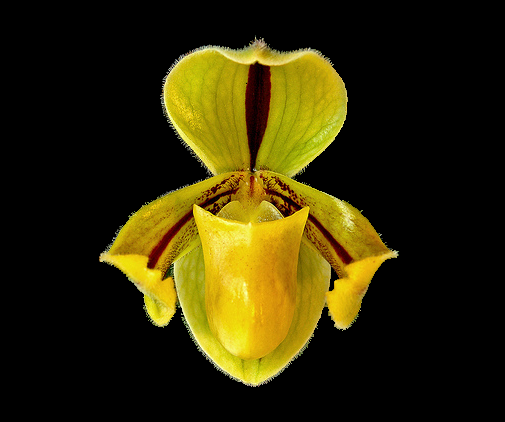
\includegraphics[width=0.5\linewidth]{grabcut_output}
    \endminipage
    \caption{Foreground segmentation with the GrabCut algorithm. The image on the left displays how the initial region of interest is set during automated feature extraction. Photo of \textit{Paphiopedilum druryi} by Peter Tremain.}
    \label{fig:grabcut-output}
\end{figure*}

BGR colour data were extracted and used as features for training the neural networks. This was done by calculating the up-right bounding square for the main contour, dividing the square into $N$ equal horizontal and vertical sections (bins), and calculating the mean blue, green, and red colour intensity for each bin (figure~\ref{fig:bgr-means-sections}). A histogram of the mean BGR colour intensities  shows that this basic feature captures some information about flower shape as well (figure~\ref{fig:bgr-means-plots}).

\begin{figure}[h]
    \centering
    \includegraphics[width=0.5\textwidth]{bgr_means_sections}
    \caption{The first horizontal and vertical bin ($N~=~20$) is highlighted in a foreground segmented image of \textit{P.~druryi}.}
    \label{fig:bgr-means-sections}
\end{figure}

\begin{figure*}[h]
    \centering
    \includegraphics[width=\textwidth]{bgr_means_plots}
    \caption{Plots of the mean BGR colour intensities for an image of \textit{P. druryi}. The plots display the mean intensities for the horizontal and vertical bins respectively.}
    \label{fig:bgr-means-plots}
\end{figure*}

\subsection{Neural network training}

Several artificial neural network training routines were developed and released as a separate Python package called NBClassify (\url{https://github.com/naturalis/nbclassify/nbclassify}).

\subsection{Cross-validation}

Stratified k-folds cross-validation was performed to estimate the accuracy of the classifiers. Species names were used to set the classes for the cross-validations. In order to include all species, the number of folds was set to 4 (k=4). Cross-validation was also performed with 10 folds, only including the species represented by at least k=10 photos.

Principal components analysis (PCA) was performed on the training data to assess the suitability of the features to differentiate the photos by genus, section, and species.

\section{Results}
\label{sect:results}

\subsection{Reference photo collection}

In total {\PhotoCount} photos for {\SpeciesCount} species were collected (table~\ref{tbl:photo-counts}). The collection contains photos for the genera \textit{Cypripedium}, \textit{Mexipedium}, \textit{Paphiopedilum}, \textit{Phragmipedium}, and \textit{Selenipedium}. With the number of photos for the five genera ranging from just 4 for the genus \textit{Selenipedium} to 888 for \textit{Paphiopedilum}, the collection is highly unbalanced.

\begin{table}[h]\footnotesize
    \caption{The number of photos collected per genus, as well as the number of sections and species per genus represented by the photo collection.}
    \begin{center}
    \begin{tabular}{llll}
    \toprule
    \textbf{Genus} & \textbf{Section} & \textbf{Species} & \textbf{Photos} \\
    \midrule
    \input{table-taxa-summary.inc}
    \bottomrule
    \end{tabular}
    \end{center}
    \label{tbl:photo-counts}
\end{table}

\subsection{Image feature extraction}

The \verb/color_bgr_means/ method from ImgPheno extracts the BGR colour intensities from a region of interest in an image. This feature has a parameter, \verb/bins/, which is used to set the number of horizontal and vertical sections in which to divide the image. The method returns for each section the mean intensity for each of the components of the BGR colour space (blue, green, and red) (figure~\ref{fig:bgr-means-plots}).

\subsection{Cross-validation}

Stratified k-folds cross-validation was performed to estimate the accuracy of the classifiers. The accuracy for genus classification was 75\%, but accuracy drops dramatically as section (52\%) and species (48\%) are also included in the classification (table~\ref{tbl:x-validation-results}). With 10 folds and including only those species for which at least 10 photos are collected, results in slightly better accuracies (table~\ref{tbl:x-validation-results}), but this can probably be attributed to the reduced number of sections and species.

Principal components analysis (PCA) with orthogonal rotation (varimax) was conducted on training training data for genus classification containing -1 to 1 scaled mean colour intensities for the BGR colour space with 20 horizontal and vertical bins, which translates to 120 features. The Kaiser-Meyer-Olkin measure verified the sampling adequacy for the analysis with an overall Measure of Sampling Adequacy (MSA) of 0.92, and all MSA values for individual items were >0.76, which is well above the acceptable limit of 0.5. Bartlett's test of sphericity $\chi^2 (7140) = 452642$, $p = 0$, indicated that correlations between items were sufficiently large for PCA. An initial PCA was run to obtain eigenvalues for each component in the data. The scree plot constructed from the eigenvalues showed inflexion that would justify retaining 3 components (explaining 65\% of the variance). Given the large sample size (N = 1134) and the convergence of the scree plot, 3 components were retained in the final analysis. The same PCA workflow was repeated for training data for section classification within the genus Paphiopedilum, and for species classification within the section Parvisepalum of genus Paphiopedilum. Figure~\ref{fig:pca-plots} shows the scatter plots for the principal components.

\begin{table}[h]\footnotesize
    \caption{Results for stratified k-fold cross-validations. Cross-validation was performed on three taxonomic ranks: genus, section, and species. The results for genus/section and genus/section/species combine the results from their respective ranks.}
    \begin{center}
    \begin{tabular}{lp{1.5cm}p{1.5cm}}
    \toprule
    \textbf{Classification} & \textbf{Accuracy (k=4)} & \textbf{Accuracy (k=10)} \\
    \midrule
    genus                   & 75\%    & 81\% \\
    section                 & 52\%    & 60\% \\
    species                 & 48\%    & 56\% \\
    genus/section           & 41\%    & 49\% \\
    genus/section/species   & 20\%    & 27\% \\
    \bottomrule
    \end{tabular}
    \end{center}
    \label{tbl:x-validation-results}
\end{table}

\section{Conclusions and discussion}
\label{sect:conclusion}

In an effort the normalize images prior to feature extraction, some colour image enhancement methods developed by \citet{Naik2003} were implemented. Most images used were already of good quality, and performing hue-preserving linear transformation with maximum contrast often did not result in an enhanced image, and thus colour enhancement using this method did not result in improved identification accuracy. Several feature extraction method were implemented in the ImgPheno package, including methods for obtaining image moments based shape characteristics, methods for getting contour outline characteristics (e.g. convex area, eccentricity, equivalent diameter, extent, orientation, perimeter, solidity), specialised shape description methods, and methods for obtaining colour data. This study builds on a simple features extraction method for obtaining colour data, \verb/color_bgr_means/.

% Need more and better photo material.
% Better feature extraction methods.

\lipsum[1]

\section*{Acknowledgements}

% De namen van alle fotografen in de format J.H. Simpson.

\lipsum[1]

%% If you have bibdatabase file and want bibtex to generate the
%% bibitems, please use
%%
%%  \bibliographystyle{elsarticle-num}
%%  \bibliography{<your bibdatabase>}

%% else use the following coding to input the bibitems directly in the
%% TeX file.

\section*{References}

%% APA style with "Author, year" format.
\bibliographystyle{apa}
\biboptions{authoryear}

\bibliography{references}

%% The Appendices part is started with the command \appendix;
%% appendix sections are then done as normal sections
\appendix
\onecolumn

\section{Metadata database}
\label{sect:meta-database}

\begin{figure*}[!h]
    \centering
    \includegraphics[width=\textwidth]{meta_database_diagram}
    \caption{Diagram of the metadata database used for storing taxonomic information for a collection of reference photos. Diagram created with SchemaCrawler (\url{http://schemacrawler.sourceforge.net}).}
    \label{fig:meta-database}
\end{figure*}

\section{Reference photo collection}
\label{sect:reference-photo-collection}

\begin{footnotesize}
\begin{longtable}{llllll}
    \caption{Taxa represented by the reference photo collection and the number of photos for each species.}
    \label{tbl:taxa-stats}
    \endfirsthead
        \caption*{\textbf{Table \ref{tbl:taxa-stats}.} (continued)}
        \\\textbf{Taxa} & \textbf{Photos} \\
        \midrule
    \endhead
        %\midrule
        \caption*{\footnotesize\textit{(continued on next page)}}
    \endfoot
        \bottomrule
    \endlastfoot

    \toprule
    \textbf{Taxa} & \textbf{Photos} \\
    \midrule
    \input{table-taxa.inc}
\end{longtable}
\end{footnotesize}

\clearpage
\section{Scatter plots for principal components analyses}
\label{sect:pca-plots}

\begin{figure}[!h]
    \minipage{\textwidth}
        \includegraphics[width=0.5\linewidth]{genus_pca_plot}
        \includegraphics[width=0.5\linewidth]{{{Cypripedium.section_pca_plot}}}
    \endminipage
    \par\vfill
    \minipage{\textwidth}
        \includegraphics[width=0.5\linewidth]{{{Paphiopedilum.section_pca_plot}}}
        \includegraphics[width=0.5\linewidth]{{{Paphiopedilum.Parvisepalum.species_pca_plot}}}
    \endminipage
    \caption{Scatter plots for the principal components analysis results. PCA was conducted on training data for genus classification, \textit{Cypripedium} section classification, \textit{Paphiopedilum} section classification, and \textit{Paphiopedilum} section \textit{Parvisepalum} species classification. For all plots the first principal component (PC1) was plotted against the second (PC2).}
    \label{fig:pca-plots}
\end{figure}

\end{document}
